\documentclass[10pt]{article}
\usepackage{icmlko}

\icmlmeta{IP 파운데이션 월드모델}{501}{정정본 --- 스텝 500 의 제목이 틀렸다}{「이득의 전부가 도메인 사이」의 근거는 분해가 아니라 표본 크기 실험이었다. 그리고 그 자리에 들어갈 수도 0 과 못 가른다}

\begin{document}

\twocolumn[
\icmlheader

\begin{abstract}
\textbf{이것은 스텝 500 의 정정본이다.} 500 은 「층 ③(무관 배경)의 이득 $+$0.0598 의
\emph{전부}가 도메인 \emph{사이}의 것」이라 주장했고 그 문장을 제목에 실었다. 근거는
「쌍 가중 도메인 안 평균 $\Delta\rho=+$0.00163」 하나였다. \textbf{그 수를 만든 코드가
도메인 부분집합에서 모형을 다시 적합한다.} 도서 도메인이면 20쌍을 5겹으로 잘라
\textbf{16행으로 12열}을 적합한 뒤 「③이 안 든다」고 읽은 것이다 --- 그것은 분해가
아니라 \textbf{표본 크기 실험}이다. 옳은 자는 \textbf{팔 전량에서 한 번만 적합하고
채점만 도메인 안으로 좁히는 것}이고, 그렇게 재면 \textbf{도메인 안 이득이 $+$0.087763
으로 합산($+$0.059774)보다 크다}(1.4683배). 켄달 일치쌍을 짝 단위로 가르면
\textbf{안쪽 몫이 43.62\,\%} 이고 \textbf{짝당으로는 안쪽이 바깥쪽의 2.10배}다.
\textbf{그러므로 「전부 도메인 사이」를 철회한다.} \textbf{그런데 그 자리에 새 헤드라인을
놓을 수도 없다} --- $+$0.087763 에 군집 부트스트랩 SE 를 붙이면 $0.044957$ 이고
$T=0.089915$ 라 \textbf{「못 가른다」}이며 95\,\% 구간 $[-0.0051,\;+0.1720{]}$ 이 0을
품는다. \textbf{살아남는 문장은 하나다: 「③의 정보는 도메인 이름표로 \emph{대체 가능}
하다」} --- 도메인 지시자만 넣으면 $+$0.087630 을 벌고 그 위에서 ③은 $-$0.007503 이다.
덤으로 \textbf{500 의 반증조건이 구성상 도달 불가능}했음을 보이고 도달 가능한 것으로
바꿨다.
\end{abstract}
]

\begin{figure*}[t]
\centering
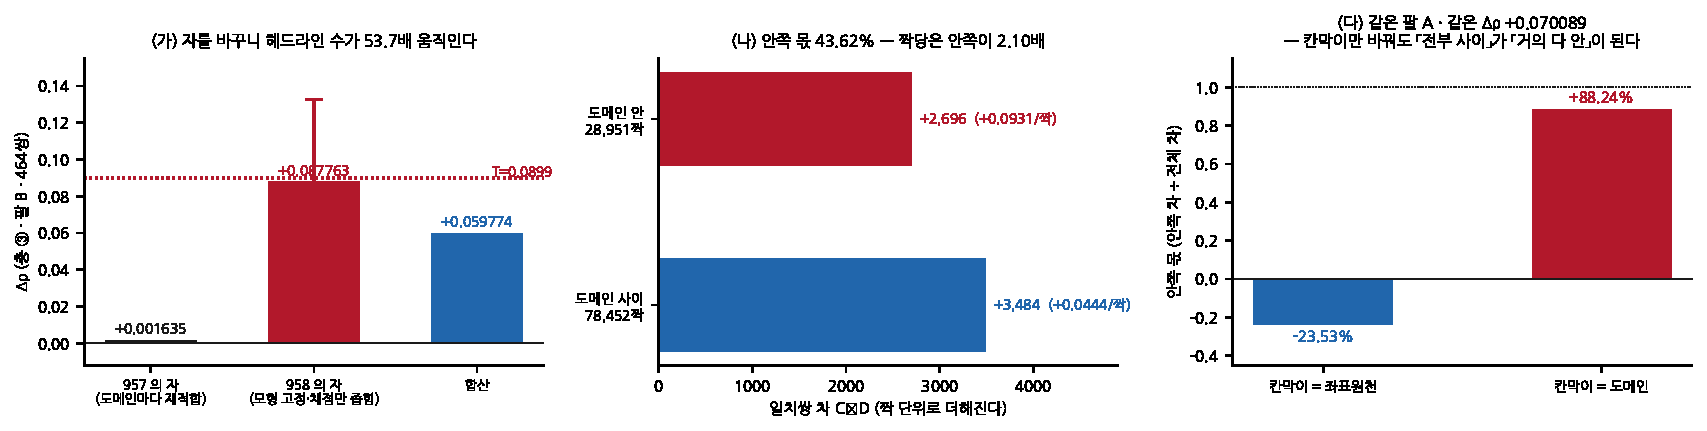
\includegraphics[width=\textwidth]{figs/ret.pdf}
\caption{(가) 같은 자료·같은 물음인데 \emph{자}를 바꾸니 헤드라인 수가 53.7배 움직인다.
빨간 막대의 오차막대가 $\pm$SE, 점선이 문턱 $T$ --- \textbf{새 수도 $T$ 를 못 넘는다}.
(나) 켄달 일치쌍은 짝 단위로 더해지므로 「안 $+$ 사이 $=$ 전체」가 항등이다. 바깥쪽이
총량에서 앞서는 것은 \textbf{짝이 2.71배 많아서일 뿐}이고 짝당으로는 안쪽이 2.10배다.
(다) 같은 팔·같은 $\Delta\rho$ 인데 \textbf{칸막이만 바꾸면} 안쪽 몫이 $-$23.5\,\% 에서
$+$88.2\,\% 로 뒤집힌다.}
\end{figure*}

\section{무엇이 틀렸나}

스텝 500 의 주장은 두 문장이었고 \textbf{둘은 다른 주장인데 논문이 강한 쪽을 실었다}.

\begin{itemize}
\item[(가)] 「③의 이득의 \emph{전부}가 도메인 사이의 것이다」 --- \textbf{틀렸다.}
\item[(나)] 「③의 정보는 도메인 이름표로 \emph{대체 가능}하다」 --- \textbf{맞다.}
\end{itemize}

(가)의 근거는 도메인별 $\Delta\rho$ 를 쌍으로 가중해 더한 $+$0.00163 하나다. 그 수를
만든 줄이 \verb|dom[dm] = one(rows, ["x1"], ["x3"], "개체")| 인데, \verb|one| 이
\verb|rho_of| 를 부르고 \verb|rho_of| 가 \verb|oof| 를 부른다 --- 즉 \textbf{도메인
부분집합에서 능형회귀를 처음부터 다시 적합한다}. 도메인별 훈련 행 수는 도서 16,
모바일·웹툰·팝업 19, 시장팝업 28, 세계애니 176 이고 \textbf{열은 전부 12} 다.

\claimx{$+$0.00163 은 「도메인 안에서 ③이 더하는가」의 답이 아니다. 「20$\sim$220행으로
훈련해도 ③을 배울 수 있는가」의 답이다 --- \textbf{분해가 아니라 표본 크기 실험}이다.
같은 자로 팔 A 를 재면 원천별 $-$0.0719 와 $-$0.2764 가 나오는데 이 둘은 26행·13행에서
적합한 \emph{서로 다른 추정량}이라 합산 $+$0.0701 과 애초에 같은 자가 아니다.}{이
주장은 「도메인마다 다시 적합해도 고정 모형과 같은 수가 나온다」로 죽는다. 실측은
$+$0.001635 대 $+$0.087763 --- \textbf{53.7배} 차다.}

\section{정본 자 --- 모형을 고정하고 채점만 좁힌다}

팔 전량(464쌍)에서 \textbf{한 번만} 적합해 OOF 예측 두 벡터 $P_\text{①}$,
$P_\text{①+③}$ 을 얻고, 그 뒤로는 다시 만들지 않는다. 도메인 $g$ 마다
$\rho_g=\mathrm{spearman}(P[g],y[g])$ 를 내고 쌍으로 가중해 더한다. 분자
$40.45895898482041$, 분모 $461$ 쌍(아이돌 3쌍은 20 미만이라 뺐다).

\textbf{배선 검사가 이것을 센다} --- 채점 루프에서 \verb|ridge_fit| 호출 수가
\textbf{0}이다(세 팔 전부). 「고정했다」를 산문으로 쓰지 않고 계수기로 신고한다.

켄달 일치쌍은 스피어만과 달리 \textbf{짝 단위로 더해지므로} 안/사이가 항등으로 갈린다:
도메인 안 28{,}951짝 $\to$ $+$2{,}696($+$0.093123/짝), 도메인 사이 78{,}452짝 $\to$
$+$3{,}484($+$0.044409/짝), $y$ 동점 13짝. 셋을 더하면 $107{,}416=\binom{464}{2}$ 다.

\claimx{층 ③의 이득은 도메인 안에도 있다. 고정 모형·쌍 가중 안쪽 $\Delta\rho$ 가
$+$0.087763 으로 합산 $+$0.059774 의 1.4683배이고, 켄달 안쪽 몫이 43.62\,\%,
짝당으로는 안쪽이 바깥쪽의 2.10배다. \textbf{따라서 「전부 도메인 사이」를 철회한다.}}
{안쪽 몫이 15\,\% 미만이거나 안쪽 $\Delta\rho$ 가 합산의 10\,\% 미만이면 죽는다.
$N_{\min}\in\{1,10,20\}$ 셋 다 살아남았다.}

\section{그런데 새 헤드라인도 못 세운다}

500 의 진짜 병은 자가 틀린 것보다 \textbf{결론이 걸린 수에만 불확실도가 없었던} 것이다.
그래서 정정본은 새 수에 먼저 SE 를 붙인다. 군집(개체 462) 부트스트랩 2{,}000회 전부 성공.

\begin{center}\small
\begin{tabular}{lr}
\toprule
$\Delta\rho_\text{안쪽}$ & $+$0.087763 \\
$\mathrm{SE}_\text{boot}$ & 0.044957 \\
$T=\max(0.00353,\,2\mathrm{SE})$ & 0.089915 \\
95\,\% 구간 & $[-0.005067,\;+0.171975]$ \\
\midrule
판정 & \textbf{못 가른다} \\
\bottomrule
\end{tabular}
\end{center}

\claimx{\textbf{500 의 헤드라인도 501 의 헤드라인 후보도 둘 다 0 과 못 가르는 수다.}
$|+0.087763|\le T=0.089915$ 이고 95\,\% 구간이 0 을 품는다. 군집 열을 도메인으로
바꿔도(SE 0.065770) 판정이 안 바뀐다. \textbf{틀린 문장을 옳은 문장으로 갈아 끼우는
정정이 아니라, 그 자리에 설 수 있는 문장이 없다는 것이 이 정정본의 결론이다.}}
{$2\mathrm{SE}<|\Delta\rho|$ 가 되면 죽는다. 쌍을 464 에서 $\sim$490 으로만 늘려도
경계에 닿는다 --- \textbf{도달 가능한 반증조건이다}.}

\section{그래서 무엇이 살아남나}

\begin{center}\small
\begin{tabular}{lrrl}
\toprule
 & $\Delta\rho$ & $T$ & 판정 \\
\midrule
① $\to$ $+$도메인 지시자 & $+$0.087630 & 0.052078 & \textbf{든다} \\
①$+$지시자 $\to$ $+$③   & $-$0.007503 & 0.006551 & \textbf{뺀다} \\
\bottomrule
\end{tabular}
\end{center}

도메인 이름표(원-핫 9열)만 넣으면 ③이 버는 것과 \textbf{거의 같은 값}을 벌고
($+$0.087630 대 $+$0.087763) 그 위에서 ③은 해롭다.

\claimx{③의 정보는 도메인 이름표로 \textbf{대체 가능}하다. 이것은 「전부 도메인 사이의
것」과 \emph{다른 주장}이며, 자료가 지지하는 것은 이쪽까지다. 처방: 층 ③을 쓸 자리에
도메인 지시자 9열을 쓰면 같은 값을 더 싸게 얻는다.}{①$+$지시자 위에서 ③이 「든다」로
바뀌면 죽는다. 이 측정은 사후가 아니라 \textbf{사전등록된} 것이다 --- 500 은 이 자를
사후로 냈다.}

\section{500 이 안 본 것 --- 안/사이는 칸막이의 성질이다}

정정하다 새로 나온 것이 하나 있다. 팔 A(쌍 39)의 $\Delta\rho=+$0.070089 을
\textbf{칸막이만 바꿔} 갈랐다.

\begin{center}\small
\begin{tabular}{lrrr}
\toprule
칸막이 & 안쪽 짝 & 안쪽 차 & 안쪽 몫 \\
\midrule
좌표원천 & 400 & $-$8  & $-$23.53\,\% \\
도메인   & 470 & $+$30 & $+$88.24\,\% \\
\bottomrule
\end{tabular}
\end{center}

\claimx{「이 이득은 안의 것인가 사이의 것인가」는 자료의 성질이 아니라 \textbf{내가 그은
칸막이의 성질}이다. 같은 수가 「전부 사이」도 되고 「거의 전부 안」도 된다. 그러므로
$\Delta\rho$ 의 within/between 분해를 실을 때는 \textbf{어느 칸막이인가를 수와 같은 줄에}
적어야 한다.}{두 칸막이가 같은 부호·같은 크기를 내면 죽는다. 실측은 $-$23.53\,\% 대
$+$88.24\,\% 다.}

한편 팔 A 는 \textbf{어느 자로도 판정이 안 난다}($\mathrm{SE}$ 0.179004,
$T$ 0.358007). 500 이 「원리상 못 가른다」라 적은 것은 옳았고 501 이 다른 자로 확인했다.

\section{반증조건을 도달 가능하게 고친다}

500 의 반증조건은 \emph{「어느 한 도메인 안에서 $\Delta\rho>T$ 면 주장이 좁아진다」}
였는데, 도메인마다 다시 적합하면 작은 도메인의 $T$ 가 \textbf{0.088$\sim$0.173} 이라
20$\sim$24쌍으로는 \textbf{원리상 못 넘는다} --- \textbf{구성상 도달 불가능한 반증조건은
반증조건이 아니다}. 501 은 전량 적합의 $T$(0.089915)와 짝 단위 항등(15\,\% 문턱)으로
바꿨고, 둘 다 실제로 발화했다.

\section{한계}

씨앗 10개·5겹·알파 격자는 500 과 같게 두었다 --- 바꾸면 비교가 깨진다. 따라서 이 정정본은
\textbf{그 셋에 대해 견고성을 안 쟀다}. 입력은 500 이 실제로 쓴 blob 을 얼려
(압축을 푼 내용 sha256 15/15 일치) 다시 읽었고, 상시 수집 데몬을 재운 채 쟀다 ---
500 은 측정 중에 데몬이 입력 11개를 다시 쓰는 일을 겪었다.

\end{document}
